% Created 2021-11-30 Tue 08:25
% Intended LaTeX compiler: pdflatex
\documentclass[presentation,aspectratio=169]{beamer}
\usepackage[utf8]{inputenc}
\usepackage[T1]{fontenc}
\usepackage{graphicx}
\usepackage{grffile}
\usepackage{longtable}
\usepackage{wrapfig}
\usepackage{rotating}
\usepackage[normalem]{ulem}
\usepackage{amsmath}
\usepackage{textcomp}
\usepackage{amssymb}
\usepackage{capt-of}
\usepackage{hyperref}
\usepackage{khpreamble}
\DeclareMathOperator{\atantwo}{atan2}
\usetheme{default}
\author{Kjartan Halvorsen}
\date{\today}
\title{Sensitivity and robustness}
\hypersetup{
 pdfauthor={Kjartan Halvorsen},
 pdftitle={Sensitivity and robustness},
 pdfkeywords={},
 pdfsubject={},
 pdfcreator={Emacs 26.3 (Org mode 9.4.6)}, 
 pdflang={English}}
\begin{document}

\maketitle

\section{Intro}
\label{sec:org4453306}


\section{The sensitivity function}
\label{sec:org37d7547}


\begin{frame}[label={sec:org140e392}]{Sensitivity and complementary sensitivity}
\small

\begin{center}
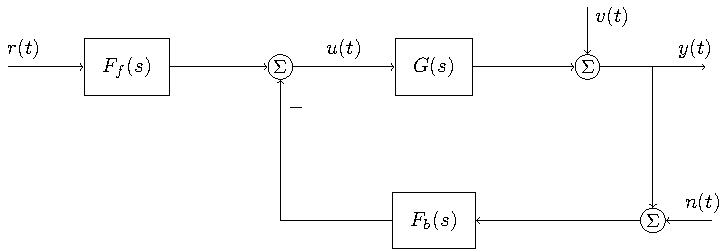
\includegraphics[width=0.8\linewidth]{../../figures/2dof-block-complete}
\end{center}
\pause
\begin{enumerate}
\item Determine the closed-loop transfer function \(G_v(s)\) from \(v(t)\) to \(y(t)\) and the transfer function \(G_n(t)\) from \(n(t)\) to \(y(t)\).
\end{enumerate}
\pause
\begin{enumerate}
\setcounter{enumi}{1}
\item Show that if \(F_{fb}(s)\) and/or \(G(s)\) contains an integrator (pole in the origin), then \(G_v(0) = 0\) and \(G_n(0) = -1\). This means that constant disturbances are completely eliminated, but a constant measurement error (sensor bias) is passed unattenuated to the output.
\end{enumerate}
\end{frame}

\begin{frame}[label={sec:org08e019f}]{The Nyquist plot and stability margins}
\begin{center}
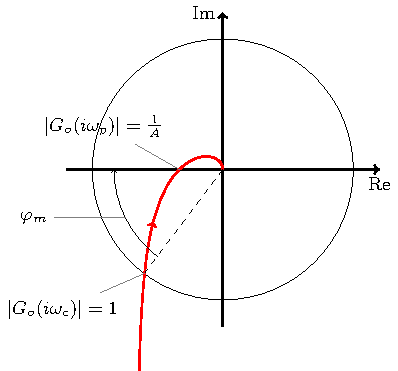
\includegraphics[width=0.4\linewidth]{../../figures/implane-nyquist-margins}
\end{center}
\end{frame}


\begin{frame}[label={sec:org7251ce2}]{The sensitivity function}
\begin{center}
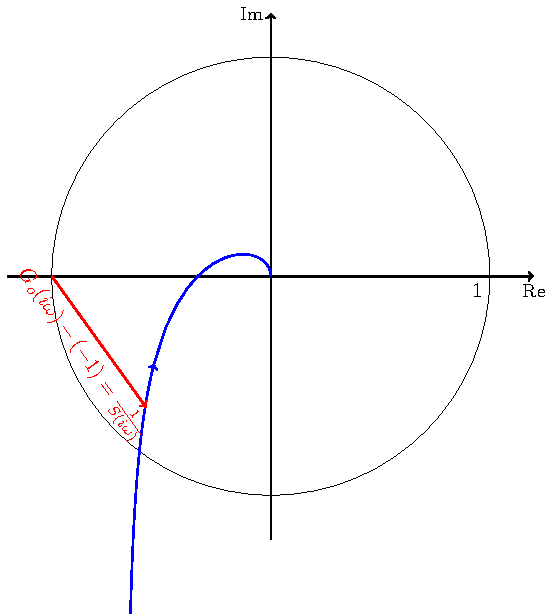
\includegraphics[width=0.4\linewidth]{../../figures/implane-sensitivity}
\end{center}

\[ S(i\omega) = G_v(i\omega) = \frac{1}{ 1 + G_o(i\omega)} = \frac{1}{1 + G(i\omega)F_{fb}(i\omega)} \]
\end{frame}




\begin{frame}[label={sec:orgeec76bd}]{The sensitivity function}
\begin{center}
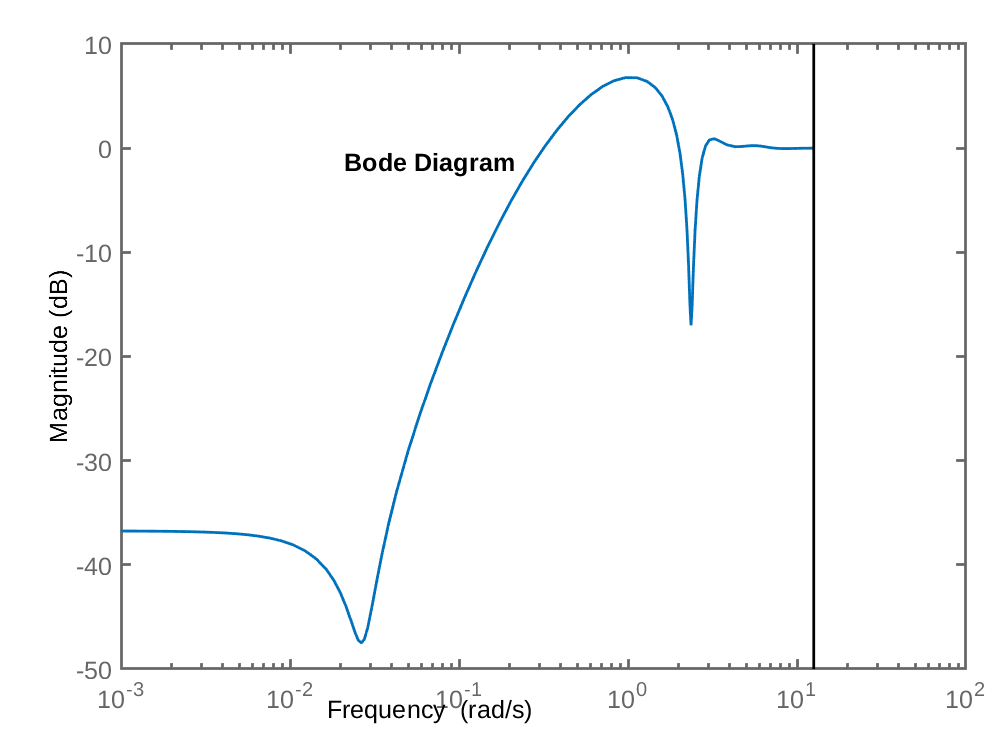
\includegraphics[width=0.7\linewidth]{../../figures/sensitivity-example}
\end{center}
\end{frame}


\section{Stein}
\label{sec:orgace975b}

\begin{frame}[label={sec:orgb1d669d}]{Interpretations of the sensitivity function}
Several important interpretations of the sensitivity function \(S(s)\)
\begin{enumerate}
\item \(S(i\omega)\) tells us how well our closed-loop system attenuates disturbances of different frequencies
\item Its maximum value is a measure of how close the closed-loop system is to being unstable.
\item \(S(i\omega)\) tells us how modelling errors or modelling variations of the plant influences the closed-loop system
\end{enumerate}
\end{frame}



\begin{frame}[label={sec:orgee41180}]{An important limitation}
\begin{center}

\includegraphics[width=0.5\linewidth]{../../figures/Stein-title.png}
\end{center}
\end{frame}


\begin{frame}[label={sec:orgc23a577}]{An important limitation}
\begin{center}
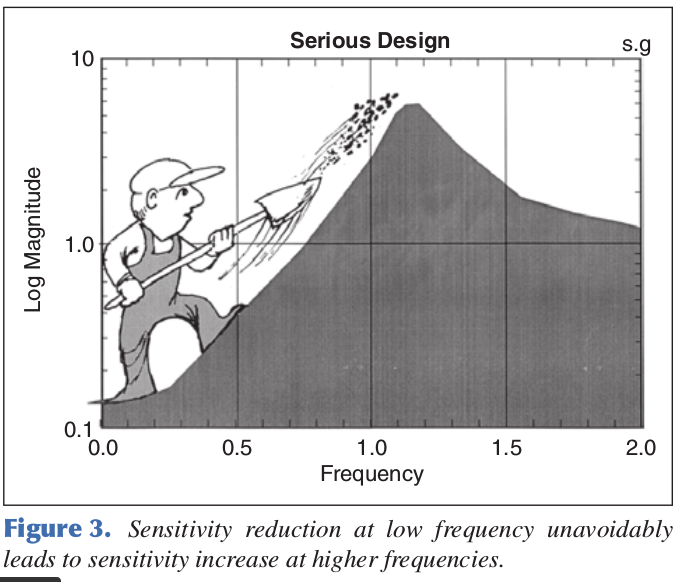
\includegraphics[width=0.5\linewidth]{../../figures/stein-serious-design.png}
\end{center}

\[ \int _{0}^{\infty }\ln |S(i\omega )|d\omega =\int _{0}^{\infty }\ln \left|{\frac {1}{1+G_o(i\omega )}}\right|d\omega =\pi \sum Re(p_{k}) \]
\end{frame}

\begin{frame}[label={sec:org16d9c7b}]{An important limitation}
\begin{center}
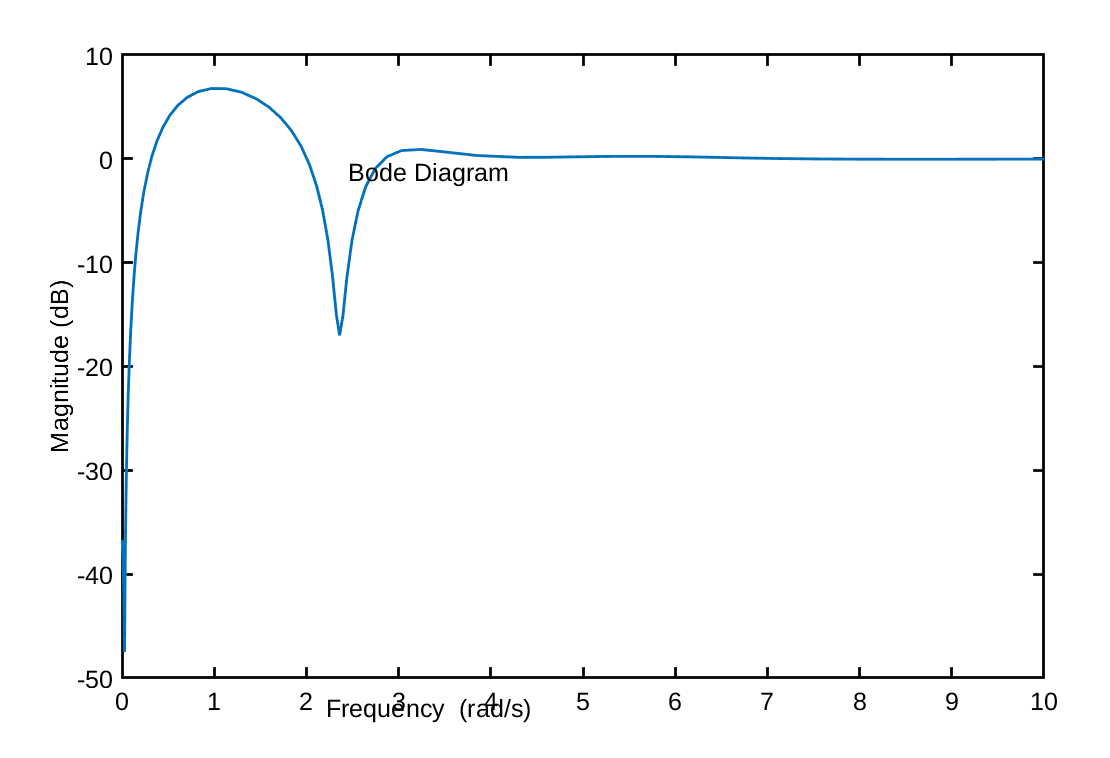
\includegraphics[width=0.6\linewidth]{../../figures/sensitivity-linear.png}
\end{center}
\end{frame}
\section{Robustness}
\label{sec:orga013b17}
\end{document}